\newpage
\section*{SINGLE FILE LOCATION}
% \parskip=0.3em
Files are an old and established mechanism used by applications to store and retrieve configuration, libraries, state, data etc. Most applications use files in their own unique manner and store files in various locations.
\begin{center}
\ding{118} \ding{118} \ding{118}
\end{center}

\textbf{Having such an extensive use of files can cause system administrators to have difficulty in finding the files necessary for their tasks during the life cycle of an application. Especially so if the files are dispersed over different folders or hidden in system-folders of the Operating System. System administrators also want to be able to perform version control on the files, having files files spread  over the whole disk practically negates to ability to perform versioning and baselining of the configuration of an application.}\\

\textit{Special cases that cause much aggravation:}
\begin{itemize}
\item Distributed Applications.\\
Many applications consist of different subsystems, which often require  subsystem-specific administration tasks. These subsystems are in many cases developed by different teams, resulting in dispersed groups of similar artifacts for each subsystem. This situation is well suited for developers as they can work in parallel. During deploy or system administration activities 
\item Hard-coded Locations.\\
This is the case when the developers put the location of the configuration files in source code and provide no parameters or interface to influence this location. This means the path can only be changed by building and deploying a new version of the application. Running multiple instances of a program on a machine with different parameters is effectively blocked by this approach. Additionally it can pose security risks if the file location is in a privileged location such as \verb|C:\Program Files| for Windows based systems.
\item Non Human Readable Configuration Files.\\
When an application provides a Graphical User Interface for configuring the application, it happens that such an application stores the captured configuration in a non human readable file. The disadvantage of this approach is that the system administrator can only see the configuration by starting the application and opening the dialogue to see the settings. This also blocks automation of deploy and install scripts and integration with automatic deploy tooling such as Puppet or Chef.
\end{itemize}

\begin{center}
\ding{118} \ding{118} \ding{118} 
\end{center}

\textbf{Therefore: Put all related files in one (hierarchical) location. Make the path of this location configurable.}\\

\begin{figure}[h]
\centering
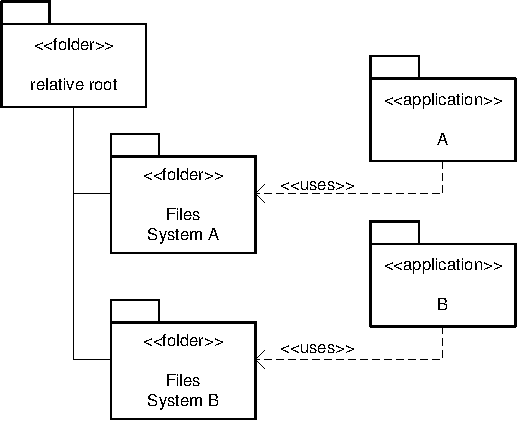
\includegraphics{patterns/singleFileLocationDiagram-01.pdf}
\caption{Basic example}
\label{fig:singleFileLocationDiagram-01}
\end{figure}

Files that logically belong together and should be at the same location are: the binaries of a system, the configuration files and the data files. In the case of log files one should first consider to {\sc Use Built-in System Logging}.

%The physical view of software architecture as described by Philippe Kruchten \cite{Kruchten1995}... todo: describe that this view often sees subsystems or applications as a whole. It does not offer the flexibility of freely choosing the location or, even better, show that this does not have to be a fixed location but could be configurable.
 
\begin{center}
\ding{118} \ding{118} \ding{118} 
\end{center}

\textit{Rationale.}\\
Without using this pattern the files of applications will be dispersed over several distinct locations which makes it hard to maintain the application. When a file of a module isn't used anymore it will easily remain in disuse and get overlooked which causes pollution of your hard disk.

\begin{figure}[h]
\centering
%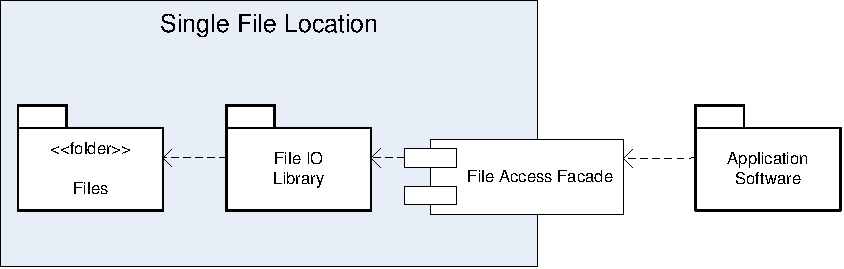
\includegraphics{patterns/singleFileLocationDiagram-02.pdf}
\caption{Another example}
\label{fig:singleFileLocationDiagram-02}
\end{figure}
